\lab{Gibbs Sampling and LDA}{Gibbs Sampling and LDA}
\objective{Understand the basic principles of implementing a Gibbs sampler. Apply this to Latent Dirichlet Allocation.}

\section*{Gibbs Sampling}
Gibbs sampling is an MCMC sampling method in which we construct a Markov chain which is used to sample from a desired joint (conditional) distribution
\begin{equation*}
\mathbb{P}(x_{1},\cdots,x_{n} \mid \mathbf{y}).
\end{equation*}
Often it is difficult to sample from this high-dimensional joint distribution, while it may be easy to sample from the one-dimensional
conditional distributions
\begin{equation*}
\mathbb{P}(x_{i} \mid \mathbf{x}_{-i}, \mathbf{y})
\end{equation*}
where $\mathbf{x}_{-i} = x_{1},\cdots,x_{i-1},x_{i+1},\cdots,x_{n}.$

\begin{algorithm}
\begin{algorithmic}[1]
\Procedure{Gibbs Sampler}{}
    \State \textrm{Randomly initialize } $x_1,x_2,\ldots,x_n$.
    \For{$k = 1, 2, 3, \ldots$}
        \For{$i = 1, 2, \ldots,n$}
            \State \textrm{Draw } $x \sim \mathbb{P}(x_{i} \mid \mathbf{x}_{-i}, \mathbf{y})$
            \State \textrm{Fix } $x_i = x$
        \EndFor
        \State $\mathbf{x}^{(k)}= (x_1,x_2,\ldots,x_n)$
    \EndFor
\EndProcedure
\end{algorithmic}
\caption{Basic Gibbs Sampling Process.}
\label{alg:gibbs}
\end{algorithm}
A Gibbs sampler proceeds according to Algorithm \ref{alg:gibbs}.
Each iteration of the outer for loop is a \emph{sweep} of the Gibbs sampler, and the value of $\mathbf{x}^{(k)}$ after a sweep is a \emph{sample}.
This creates an irreducible, non-null recurrent, aperiodic Markov chain over the state space consisting of all possible $\mathbf{x}$.
The unique invariant distribution for the chain is the desired joint distribution
\begin{equation*}
\mathbb{P}(x_{1},\cdots,x_{n} \mid \mathbf{y}).
\end{equation*}
Thus, after a burn-in period, our samples $\mathbf{x}^{(k)}$ are effectively samples from the desired distribution.

Consider the dataset of $N$ scores from a calculus exam in the file \texttt{examscores.npy}.
We believe that the spread of these exam scores can be modeled with a normal distribution of mean $\mu$ and variance $\sigma^{2}$.
Because we are unsure of the true value of $\mu$ and $\sigma^2$, we take a Bayesian approach and place priors on each parameter to quantify this uncertainty:
\begin{align*}
\mu & \sim N(\nu, \tau^{2})\quad &&\text{(a normal distribution)} \\
\sigma^{2} & \sim IG(\alpha, \beta) &&\text{(an inverse gamma distribution)}
\end{align*}
Letting $\mathbf{y} = (y_1,\ldots,y_N)$ be the set of exam scores, we would like to update our beliefs of $\mu$ and $\sigma^2$ by sampling from the posterior
distribution
\begin{equation*}
\mathbb{P}(\mu, \sigma^{2} \mid \mathbf{y}, \nu, \tau^{2}, \alpha, \beta).
\end{equation*}
Sampling directly can be difficult. However, we \emph{can} easily sample from the following conditional distributions:
\begin{align*}
\mathbb{P}(\mu \mid \sigma^{2}, \mathbf{y}, \nu, \tau^{2}, \alpha, \beta) & = \mathbb{P}(\mu \mid \sigma^{2}, \mathbf{y}, \nu, \tau^{2})\\
\mathbb{P}(\sigma^{2} \mid \mu, \mathbf{y}, \nu, \tau^{2}, \alpha, \beta) & = \mathbb{P}(\sigma^{2} \mid \mu, \mathbf{y}, \alpha, \beta)
\end{align*}
The reason for this is that these conditional distributions are \emph{conjugate} to the prior distributions, and hence are part of the same distributional
families as the priors. In particular, we have
\begin{align*}
\mathbb{P}(\mu \mid \sigma^{2}, \mathbf{y}, \nu, \tau^{2}) &\sim N(\mu^*, (\sigma^*)^2)\\
\mathbb{P}(\sigma^{2} \mid \mu, \mathbf{y}, \alpha, \beta) &\sim IG(\alpha^*, \beta^*),
\end{align*}
where
\begin{align*}
(\sigma^*)^2 &= \left(\frac{1}{\tau^2}+\frac{N}{\sigma^2}\right)^{-1}\\
\mu^* &= (\sigma^*)^2\left(\frac{\nu}{\tau^2} + \frac{1}{\sigma^2}\sum_{i=1}^N y_i \right)\\
\alpha^* &= \alpha + \frac{N}{2}\\
\beta^* &= \beta + \frac{1}{2}\sum_{i=1}^N (y_i-\mu)^2
\end{align*}
Note that $\mu^*$ and $\left(\sigma^*\right)^2$ are \emph{not} samples and are not used to replace $\mu$ and $\sigma^2$ themselves; rather, they're parameters of the marginal distribution of $\mu$ (which happens to also be distributed normally) as shown above.

We have thus set this up as a Gibbs sampling problem, where we have only to alternate between sampling $\mu$ and sampling $\sigma^{2}$ (so using Algorithm \ref{alg:gibbs}, we would have $x_1 = \mu$ and $x_2 = \sigma^2$).
We can sample from a normal distribution and an inverse gamma distribution as follows:
\begin{lstlisting}
import numpy as np
from scipy.stats import norm
from scipy.stats import invgamma

mu = 0 # the mean
sigma2 = 9 # the variance
normal_sample = norm.rvs(mu, scale=np.sqrt(sigma))
alpha = 2
beta = 15
invgamma_sample = invgamma.rvs(alpha, scale=beta)
\end{lstlisting}
Note that when sampling from the normal distribution, we need to set the \li{scale} parameter to the standard deviation, \emph{not} the variance.

\begin{problem}
Write a function that accepts data $\y$, prior parameters $\nu$, $\tau^2$, $\alpha$, and $\beta$, and an integer $n$.
Use Gibbs sampling to generate $n$ samples of $\mu$ and $\sigma^2$ for the exam scores problem.

Test your sampler with priors $\nu=80$, $\tau^{2} = 16$, $\alpha = 3$, and $\beta = 50$, collecting $1000$ samples.
Plot your samples of $\mu$ and your samples of $\sigma^{2}$ versus the number of samples.
They should both converge quickly, so that both plots look like ``fuzzy caterpillars''.
\end{problem}

We'd like to look at the posterior marginal distributions for $\mu$ and $\sigma^2$.
To plot these from the samples, use a kernel density estimator from \li{scipy.stats}.
If our samples of $\mu$ are called \li{mu_samples}, then we can do this with the following code.
\begin{lstlisting}
import numpy as np
from matplotlib import pyplot as plt
from scipy.stats import gaussian_kde

mu_kernel = gaussian_kde(mu_samples)
x = np.linspace(min(mu_samples) - 1, max(mu_samples) + 1, 200)
plt.plot(x, mu_kernel(x))
plt.show()
\end{lstlisting}

\begin{figure}[H]
    \begin{subfigure}[b]{.49\textwidth}
        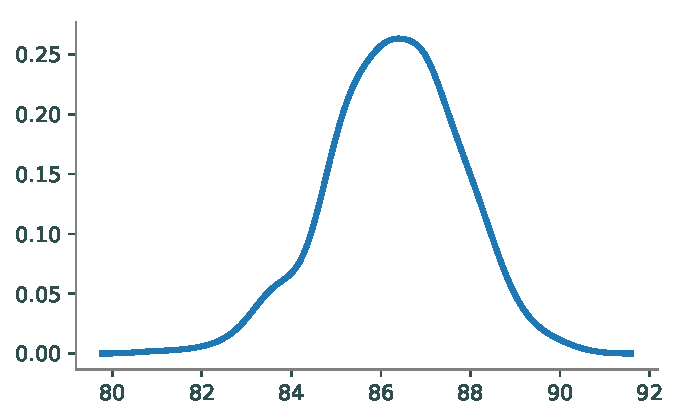
\includegraphics[width=\textwidth]{figures/mu_posterior.pdf}
        \caption{Posterior distribution of $\mu$.}
    \end{subfigure}
    \begin{subfigure}[b]{.49\textwidth}
        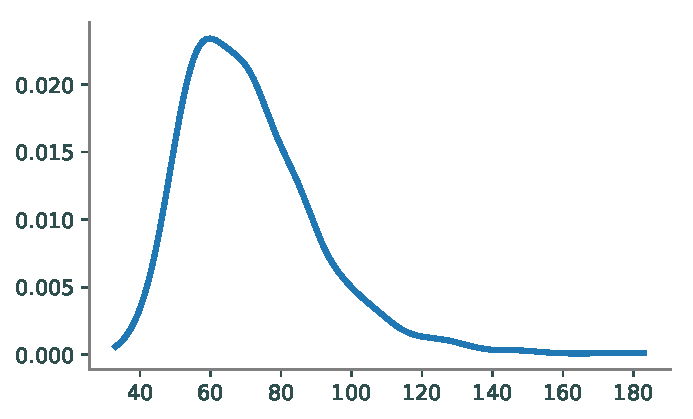
\includegraphics[width=\textwidth]{figures/sigma2_posterior.pdf}
        \caption{Posterior distribution of $\sigma^2$.}
    \end{subfigure}
\caption{Posterior marginal probability densities for $\mu$ and $\sigma^2$.}
\label{fig:post}
\end{figure}

Keep in mind that the plots above are of the posterior distributions of the \emph{parameters}, not of the scores. If we would like to compute the posterior distribution of a new exam score $\tilde{y}$ given our data $\mathbf{y}$ and prior parameters, we compute what is known as the \emph{posterior predictive distribution}:
\begin{equation*}
\mathbb{P}(\tilde{y} \mid \mathbf{y}, \lambda) = \int_{\Theta} \mathbb{P}(\tilde{y} \mid \Theta)\mathbb{P}(\Theta \mid \mathbf{y}, \lambda) d\Theta
\end{equation*}
where $\Theta$ denotes our parameters (in our case $\mu$ and $\sigma^{2}$) and $\lambda$ denotes our prior parameters (in our case $\nu, \tau^{2}, \alpha,$ and $\beta$).

Rather than actually computing this integral for each possible $\tilde{y}$, we can do this by sampling scores from our parameter samples. In other words, sample
\begin{equation*}
\tilde{y}_{(t)} \sim N(\mu_{(t)}, \sigma_{(t)}^{2})
\end{equation*}
for each sample pair $\mu_{(t)}, \sigma_{(t)}^{2}$. Now we have essentially drawn samples from our posterior predictive distribution, and we can use a kernel density estimator to plot this distribution from the samples.

\begin{figure}[H]
    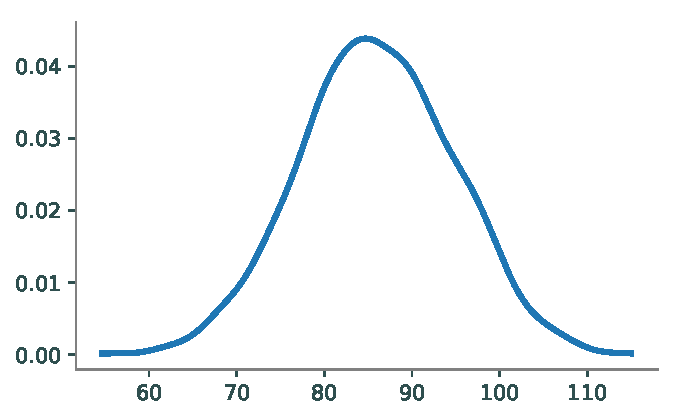
\includegraphics[width=.7\textwidth]{figures/predictiveposterior.pdf}
    \caption{Predictive posterior distribution of exam scores.}
    \label{fig:predictive}
\end{figure}

\begin{problem} % Visualize Gibbs sampler results.
Plot the kernel density estimators for the posterior distributions of $\mu$ and $\sigma^{2}$.
You should get plots similar to those in Figure \ref{fig:post}.

Next, use your samples of $\mu$ and $\sigma^{2}$ to draw samples from the posterior predictive distribution.
Plot the kernel density estimator of your sampled scores.
Compare your plot to Figure \ref{fig:predictive}.
\end{problem}

\section*{Latent Dirichlet Allocation}

Gibbs sampling can be applied to an interesting problem in natural language processing (NLP): determining which topics are prevalent in a document.
\emph{Latent Dirichlet Allocation} (LDA) is a generative model for a collection of text documents.
It supposes that there is some fixed vocabulary (composed of $V$ distinct terms) and $K$ different topics, each represented as a probability distribution $\phi_{k}$ over the vocabulary, each with a Dirichlet prior $\beta$.
This means $\phi_{k,v}$ is the probability that topic $k$ is represented by vocabulary term $v$.

With the vocabulary and topics chosen, the LDA model assumes that we have a set of $M$ documents (each ``document'' may be a paragraph or other section of the text, rather than a ``full'' document).
The $m$-th document consists of $N_m$ words, and a probability distribution $\theta_{m}$ over the topics is drawn from a Dirichlet distribution with parameter $\alpha$.
Thus $\theta_{m,k}$ is the probability that document $m$ is assigned label $k$.
If $\phi_{k,v}$ and $\theta_{m,k}$ are viewed as matrices, their rows sum to one.

\interfootnotelinepenalty=100000

We will now iterate through each document in the same manner.
Assume we are working on document $m$, which you will recall contains $N_{m}$ words.
For word $n$, we first draw a topic assignment $z_{m,n}$ from the categorical distribution $\theta_{m}$, and then we draw a word $v$ from the categorical distribution $\phi_{z_{m,n}}$. 
Throughout this implementation, we assume $\alpha$ and $\beta$ are scalars\footnote{The Dirichlet distribution Dir$(x^{}_{1},...,x^{}_s,\alpha^{}_{1},...,\alpha^{}_s)$ usually requires the parameter $\alpha$ to be a vector of length $s$, but when $\alpha$ is a scalar, it is called the ``concentration parameter'' and behaves like a vector of length $s$ whose entries are all equal to $\alpha$.}.
In summary, we have
\begin{enumerate}
    \item Draw $\phi_{k} \sim \text{Dir}(\beta)$ for $1 \leq k \leq K$.
    \item For $1 \leq m \leq M$:
    \begin{enumerate}
        \item Draw $\theta_{m} \sim \text{Dir}(\alpha)$.
        \item Draw $z_{m,n} \sim \text{Cat}(\theta_{m})$ for $1 \leq n \leq N_{m}$.
        \item Draw $v \sim \text{Cat}(\phi_{z_{m,n}})$ for $1 \leq n \leq N_{m}$.
    \end{enumerate}
\end{enumerate}

We end up with $n$ words which represent document $m$.
Note that these words are \emph{not} necessarily distinct from one another; indeed, we are most interested in the words that have been repeated the most.

This is typically depicted with graphical plate notation as in Figure \ref{fig:ldaplates}.
\begin{figure}[h]
\centering
\begin{tikzpicture}[>=stealth', dot/.style=
    {circle,fill=black,minimum size=3pt,inner sep=0pt, outer sep=-1pt} ]

\node[draw,minimum height=3.2cm, minimum width=2.1cm](r1)[]{};
\node[draw,minimum height=5cm, minimum width=2.4cm, node distance=
    .4cm](r2)[above of=r1]{};

\node[node distance=1.3cm](Nm)[below of=r1]{$1 \le n \le N_m$};
\node[node distance=2.28cm](M)[below of=r2]{$1 \le m \le M$};

\node[node distance = 2.7cm](dummy3)[left of=r1]{};
\node[draw,minimum height=2cm, minimum width=2.1cm, node distance=
    .55cm](r3)[ below of =dummy3]{};
\node[node distance=.7cm](K)[below of=r3]{$1 \le k \le K$};

\node[node distance=.6cm](dummy)[above right of =Nm]{};
\node[circle, draw,  inner sep=5pt, fill=black!25!,node distance=.4cm]
    (w)[above of=dummy]{$v$};
\node[circle, draw,  inner sep=1pt, node distance=1.3cm](z)[above
    of=w]{$z_{m,n}$};
\node[circle, draw,  inner sep=1pt, node distance=1.3cm]
    (theta)[above of=z]{$\vec{\theta}_{m}$};

\node[node distance=1.2cm, inner sep=0pt](alpha)[above of=
    theta]{$\vec{\alpha}$};

\node[node distance=.6cm](dummy2)[above right of=K]{};
\node[node distance=.35cm, circle, inner sep=1pt, draw](phi)[above
    of=dummy2]{$\vec{\phi_k}$};
\node[node distance=1.4cm, inner sep=0pt](beta)[above of = phi]{$\vec{\beta}$};

\foreach \x/\y in {alpha/theta, theta/z, z/w, beta/phi, phi/w} \draw[->](\x)--(\y);

\end{tikzpicture}
\caption{Graphical plate notation for LDA text generation.}
\label{fig:ldaplates}
\end{figure}

In the plate model, only the variables $v$ are shaded, signifying that these are the only observations visible to us; the rest are latent variables. 
Our goal is to estimate each $\phi_{k}$ and each $\theta_{m}$. 
This will allow us to understand what each topic is, as well as understand how each document is distributed over the $K$ topics. 
In other words, we want to predict the topic of each document, and also which words best represent this topic.
We can estimate these well if we know $z_{m,n}$ for each $m, n$, collectively referred to as $\mathbf{z}$. 
Thus, we need to sample $\mathbf{z}$ from the posterior distribution $\mathbb{P}(\mathbf{z} \mid \mathbf{v}, \alpha, \beta)$, where $\mathbf{v}$ is the collection of words in the text corpus. 
Unsurprisingly, it is intractable to sample directly from the joint posterior distribution. 
However, letting $\mathbf{z}_{-(m,n)} = \mathbf{z}\setminus \{z_{m,n}\}$ (so as to condition on everything except the $(m,n)$-th entry), the conditional posterior distributions
\begin{equation*}
    \mathbb{P}(z_{m,n} = k \mid \mathbf{z}_{-(m,n)}, \mathbf{v}, \alpha, \beta)
\end{equation*}
have nice, closed form solutions, making them easy to sample from.

These conditional distributions have the following form:
\begin{equation*}
\mathbb{P}(z_{m,n} = k \mid \mathbf{z}_{-(m,n)}, \mathbf{v}, \alpha, \beta) \propto \frac{\left(n_{(k,m,\cdot)}^{-(m,n)} + \alpha\right)\left(n_{(k, \cdot, v)}^{-(m,n)} + \beta\right)}{n_{(k,\cdot,\cdot)}^{-(m,n)} + V \beta}
\end{equation*}
where
\begin{align*}
n_{(k,m,\cdot)} & = \mbox{ the number of words in document $m$ assigned to topic $k$} \\
n_{(k,\cdot,v)} & = \mbox{ the number of times term $v$ is assigned to topic $k$} \\
n_{(k,\cdot,\cdot)} & = \mbox{ the number of times topic $k$ is assigned in the corpus} \\
n_{(k,m,\cdot)}^{-(m,n)} & = n_{(k,m,\cdot)} - \indicator_{z_{m,n} = k} \\
n_{(k,\cdot,v)}^{-(m,n)} & = n_{(k,\cdot,v)} - \indicator_{z_{m,n} = k} \\
n_{(k,\cdot,\cdot)}^{-(m,n)} & = n_{(k,\cdot,\cdot)} - \indicator_{z_{m,n} = k}
\end{align*}

Thus, if we simply keep track of these count matrices, then we can easily create a Gibbs sampler over the topic assignments. 
This is actually a particular class of samplers known as \emph{collapsed Gibbs samplers}, because we have collapsed the sampler by integrating out $\theta$ and $\phi$.

We have provided for you the structure of a Python object \li{LDACGS} with several methods, listed at the end of this lab.
The object defines attributes \li{n\_topics}, \li{alpha}, and \li{beta} upon initialization.
The method \li{buildCorpus()} then defines attributes \li{vocab} and \li{documents}, where \li{vocab} is a list of strings (terms), and \li{documents} is a list of dictionaries (a dictionary for each document). 
For dictionary $m$ in \li{documents}, each entry is of the form $n : v$, where $v$ is the index in \li{vocab} of the $n^{th}$ word in document $m$.

The remainder of this lab will guide you through writing several more methods in order to implement the Gibbs sampler. 
The first step is to initialize the assignments and create count matrices $n_{(k,m,\cdot)}, n_{(k,\cdot,v)}$ and vector $n_{(k,\cdot,\cdot)}$.

\begin{problem}
Complete the method \li{_initialize()} to initialize as attributes \li{n\_words}, \li{n\_docs}, the three count matrices, and the topic assignment dictionary \li{topics}.

To do this, you will need to initialize \li{nkm}, \li{nkv}, and \li{nk} to be zero arrays of the correct size.
Matrix \li{nkm} corresponds to $n_{(k,m,\cdot)}$, \li{nkv} to $n_{(k,\cdot,v)}$, and \li{nk} to $n_{(k,\cdot,\cdot)}$.
You will then iterate through each word found in each document.
In the second of these for-loops (for each word), you will randomly assign \li{k} as an integer from the correct range of topics.
Then, you will increment each of the count matrices by 1, given the values for \li{k}, \li{m}, and \li{v}, where \li{v} is the index in \li{vocab} of the $n^{th}$ word in document $m$.
Finally, assign \li{topics} as given.
\end{problem}

The next method fully outlines a sweep of the Gibbs sampler.

\begin{problem}
Complete the method \li{_sweep()}. 

To do this, iterate through each word of each document. 
The first part of this method will undo what \li{_initialize()} did by decrementing each of the count matrices by 1.
Then, call the method \li{_conditional()} to use the conditional distribution (instead of the uniform distribution used previously) to pick a more accurate topic assignment \li{k}.
Finally, repeat what \li{_initialize()} did by incrementing each of the count matrices by 1, but this time using the more accurate topic assignment.
\end{problem}

\begin{comment}
Take out this problem to make the lab easier.
We need to write the method to create the appropriate conditional distribution.

\begin{problem}
Complete the method \li{_conditional()}.
It accepts arguments $m,w$ where $m$ is the document and $w$ is an index of \li{vocab}.
Don't forget to normalize to ensure you are actually returning a distribution!
\end{problem}
\end{comment}

You are now prepared to write the full Gibbs sampler.

\begin{problem}
Complete the method \li{sample()}.
The argument \li{filename} is the name and location of a .txt file, which can be read in by the provided method \li{buildCorpus()} to build the corpus. 
Stopwords are removed if the \li{stopwords} argument is provided.
Note that in \li{buildCorpus()}, \textbf{each line of} \li{filename} \textbf{is considered a document}.

Initialize attributes \li{total\_nkm}, \li{total\_nkv}, and \li{logprobs} as zero arrays.
\li{total\_nkm} and \li{total\_nkv} will be the sums of every \li{sample\_rate}$^{th}$ \li{nkm} and \li{nkv} matrix respectively.
\li{logprobs} is of length $\text{\li{burnin} } + \text{ \li{sample\_rate} } * \text{ \li{n\_samples}}$ and will store each log-likelihood after each sweep of the sampler.

Burn-in the Gibbs sampler.
After the burn-in, iterate further for \li{n\_samples} iterations, adding \li{nkm} and \li{nkv} to \li{total\_nkm} and \li{total\_nkv} respectively, at every \li{sample\_rate}$^{th}$ iteration.
Also, compute and save the log-likelihood at each iteration in \li{logprobs} using the method \li{_loglikelihood()}.
\end{problem}

You should now have a working Gibbs sampler to perform LDA inference on a corpus.
Let's test it out on some of Ronald Reagan's State of the Union addresses, found in \texttt{reagan.txt}.
Note that in \li{reagan.txt}, each line is an entire paragraph from one of Reagan's addresses, so your Gibbs sampler will consider each paragraph as a seperate document.

\begin{problem}

Create an \li{LDACGS} object with 20 topics, letting $\alpha$ and $\beta$ be the default values.
Run the Gibbs sampler, with a burn-in of 100 iterations, accumulating 10 samples, only keeping the results of every 10th sweep with the \texttt{reagan.txt} file.
Use \texttt{stopwords.txt} as the stopwords file.

\noindent Plot the log-likelihoods. 
How many iterations did it take to burn-in?

Make sure to save the \texttt{LDACGS} object, it will be used in the next problem.
\end{problem}

We can estimate the values of each $\phi_{k}$ and each $\theta_{m}$ as follows:

\begin{align*}
    \widehat{\phi}_{k,v} & = \frac{n_{(k,\cdot,v)} + \beta}{V \cdot \beta + \sum_{v=1}^{V} n_{(k,\cdot,v)}} \\
    \widehat{\theta}_{m,k} & = \frac{n_{(k,m,\cdot)} + \alpha}{K \cdot \alpha + \sum_{k=1}^{K} n_{(k,m,\cdot)}}
\end{align*}

We have provided methods \li{phi} and \li{theta} that do this for you. We often examine the topic-term distributions $\phi_{k}$ by looking at the $n$ terms with the highest probability, where $n$ is small (say $10$ or $20$).
We have provided a method \li{topterms} which does this for you.

\begin{problem}
Using the method \li{topterms()}, examine the topics for Reagan's addresses. 
If \li{n\_topics=20} and \li{n\_samples=10}, you should get the top $10$ words that represent each of the 20 topics.
Print out all 20 topics associated 10 words. 
For the top 5 topics, decide what their top 10 words jointly represent, and come up with a label for them.
\end{problem}

We can use $\widehat{\theta}$ to find the documents (paragraphs) in Reagan's addresses that focus the most on each topic. The documents with the highest values of $\widehat{\theta}_{k}$ are those most heavily focused on topic $k$.
For example, if you chose the topic label for topic $p$ to be \emph{the Cold War}, you can find the five highest values in $\widehat{\theta_{p}}$, which will tell you which five documents (paragraphs) are most centered on the Cold War.
For your convenience, the provided method \li{toplines()} accomplishes just that by printing out the top \li{n_lines} documents corresponding to each topic.

\begin{comment}
This problem was difficult for the first cohort, and since it does not add much to the lab it has been removed.

\begin{problem}
In your above topic analysis, you should have found a topic about the Cold War and one about education. Find the five paragraphs in Reagan's addresses that most closely focus on each of these topics, according to the above method.
\end{problem}
\end{comment}

Let's take a moment to see what our Gibbs sampler has accomplished.
By simply feeding in a group of documents, and with no human input, we have found the most common topics discussed, which are represented by the words most frequently used in relation to that particular topic.
The only work that the user has done is to assign topic labels, saying what the words in each group have in common.
As you may have noticed, however, these topics may or may not be \emph{relevant} topics.
You might have noticed that some of the most common topics were simply English particles (words such as \emph{a}, \emph{the}, \emph{an}) and conjunctions (\emph{and}, \emph{so}, \emph{but}).
Industrial grade packages can effectively remove such topics so that they are not included in the results.

\newpage

\section*{Additional Material} % ==============================================

\subsection*{LDACGS Source Code} % --------------------------------------------

\begin{lstlisting}
class LDACGS:
    """ Do LDA with Gibbs Sampling. """

    def __init__(self, n_topics, alpha=0.1, beta=0.1):
        """ Initializes attributes n_topics, alpha, and beta. """
        self.n_topics = n_topics
        self.alpha = alpha
        self.beta = beta

    def _buildCorpus(self, filename, stopwords_file=None):
        """ Reads the given filename, and using any provided stopwords,
            initializes attributes vocab and documents. In this lab,
            each line of filename is considered a document.
            
            vocab is a list of terms found in filename.
            
            documents is a list of dictionaries (a dictionary for each 
            document); for dictionary m in documents, each entry is of 
            the form n:v, where v is the index in vocab of the nth word 
            in document m.
        """
        with open(filename, 'r') as infile:  # Create vocab
            doclines = [line.rstrip().lower().split(' ') for line in infile]
        n_docs = len(doclines)
        self.vocab = list({v for doc in doclines for v in doc})

        self.docs = doclines  # Save the documents for toplines()

        if stopwords_file:   # If there are stopwords, remove them from vocab
            with open(stopwords_file, 'r') as stopfile:
                stops = stopfile.read().split()
            self.vocab = [x for x in self.vocab if x not in stops]
            self.vocab.sort()
        
        self.documents = []  # Create documents
        for i in range(n_docs):
            self.documents.append({})
            for j in range(len(doclines[i])):
                if doclines[i][j] in self.vocab:
                    self.documents[i][j] = self.vocab.index(doclines[i][j])


    def _initialize(self):
        """ Initializes attributes n_words, n_docs, the three count matrices, 
            and the topic assignment dictionary topics.
                        
            Note that
            n_topics = K, the number of possible topics
            n_docs   = M, the number of documents being analyzed
            n_words  = V, the number of words in the vocabulary
            
            To do this, you will need to initialize nkm, nkv, and nk 
            to be zero arrays of the correct size.
            Matrix nkm corresponds to n_(k,m,.)
            Matrix nkv corresponds to n_(k,.,v)
            Matrix nk corresponds to n_(k,.,.)
            You will then iterate through each word found in each document.
            In the second of these for-loops (for each word), you will 
            randomly assign k as an integer from the correct range of topics.
            Then, you will increment each of the count matrices by 1, 
            given the values for k, m, and v, where v is the index in 
            vocab of the nth word in document m.
            Finally, assign topics as given.
        """
        self.n_words = len(self.vocab)
        self.n_docs = len(self.documents)
                
        # Initialize the three count matrices
        # The (k, m) entry of self.nkm is the number of words in document m assigned to topic k
        self.nkm = np.zeros((self.n_topics, self.n_docs))
        # The (k, v) entry of self.nkv is the number of times term v is assigned to topic k
        self.nkv = np.zeros((self.n_topics, self.n_words))
        # The (k)-th entry of self.nk is the number of times topic k is assigned in the corpus
        self.nk = np.zeros(self.n_topics)
        
        # Initialize the topic assignment dictionary
        self.topics = {} # Key-value pairs of form (m,n):k
        
        random_distribution = np.ones(self.n_topics) / self.n_topics
        for m in range(self.n_docs):
            for n in self.documents[m]:
                # Get random topic assignment, i.e. k = ...
                # Increment count matrices
                # Store topic assignment, i.e. self.topics[(m,n)]=k
                raise NotImplementedError("Problem 3 Incomplete")
                
                
    def _sweep(self):
        """ Iterates through each word of each document, giving a better
            topic assignment for each word.
            
            To do this, iterate through each word of each document. 
            The first part of this method will undo what _initialize() did
            by decrementing each of the count matrices by 1.
            Then, call the method _conditional() to use the conditional 
            distribution (instead of the uniform distribution used 
            previously) to pick a more accurate topic assignment k.
            Finally, repeat what _initialize() did by incrementing each of
            the count matrices by 1, but this time using the more 
            accurate topic assignment.
        """
        for m in range(self.n_docs):
            for n in self.documents[m]:
                # Retrieve vocab index for n-th word in document m
                # Retrieve topic assignment for n-th word in document m
                # Decrement count matrices
                # Get conditional distribution
                # Sample new topic assignment
                # Increment count matrices
                # Store new topic assignment
                raise NotImplementedError("Problem 4 Incomplete")

                
    def sample(self, filename, burnin=100, sample_rate=10, n_samples=10, stopwords_file=None):
        """ Runs the Gibbs sampler on the given filename. 
        
            The argument filename is the name and location of a .txt 
            file, which can be read in by the provided method _buildCorpus()
            to build the corpus. Stopwords are removed if the stopwords
            argument is provided. Note that in buildCorpus(),
            each line of filename is considered a document.
            
            Initialize attributes total_nkm, total_nkv, and logprobs as
            zero arrays.
            total_nkm and total_nkv will be the sums of every 
            sample_rate-th nkm and nkv matrix respectively.
            logprobs is of length burnin + sample_rate * n_samples
            and will store each log-likelihood after each sweep of 
            the sampler.
            
            Burn-in the Gibbs sampler. After the burn-in, iterate further 
            for n_samples iterations, adding nkm and nkv to total_nkm and 
            total_nkv respectively, at every sample_rate-th iteration.
            Also, compute and save the log-likelihood at each iteration 
            in logprobs using the method _loglikelihood().
        """
        self._buildCorpus(filename, stopwords_file)
        self._initialize()
        
        self.total_nkm = np.zeros((self.n_topics, self.n_docs))
        self.total_nkv = np.zeros((self.n_topics, self.n_words))
        self.logprobs = np.zeros(burnin + sample_rate * n_samples)
        
        for i in range(burnin):
            # Sweep and store log likelihood
            raise NotImplementedError("Problem 5 Incomplete")
        for i in range(sample_rate * n_samples):
            # Sweep and store log likelihood
            raise NotImplementedError("Problem 5 Incomplete")
            if not i % sample_rate:
                # Accumulate counts
                raise NotImplementedError("Problem 5 Incomplete")

                
    def _conditional(self, m, v):
        """ Returns the conditional distribution given m and w.
            Called by _sweep(). """
        dist = (self.nkm[:,m] + self.alpha) * (self.nkv[:,v] + self.beta) / (self.nk + self.beta * self.n_words)
        return dist / np.sum(dist)

    def _loglikelihood(self):
        """ Computes and returns the log-likelihood. Called by sample(). """
        lik = 0

        for k in range(self.n_topics):
            lik += np.sum(gammaln(self.nkv[k,:] + self.beta)) - gammaln(np.sum(self.nkv[k,:] + self.beta))
            lik -= self.n_words * gammaln(self.beta) - gammaln(self.n_words * self.beta)

        for m in range(self.n_docs):
            lik += np.sum(gammaln(self.nkm[:,m] + self.alpha)) - gammaln(np.sum(self.nkm[:,m] + self.alpha))
            lik -= self.n_topics * gammaln(self.alpha) - gammaln(self.n_topics * self.alpha)

        return lik
    
    def _phi(self):
        """ Initializes attribute phi. Called by topterms(). """
        phi = self.total_nkv + self.beta
        self.phi = phi / np.sum(phi, axis=1)[:,np.newaxis]

    def _theta(self):
        """ Initializes attribute theta. Called by toplines(). """
        theta = self.total_nkm + self.alpha
        self.theta = theta / np.sum(theta, axis=1)[:,np.newaxis]

    def topterms(self, n_terms=10):
        """ Returns the top n_terms of each topic found. """
        self._phi()
        vec = np.atleast_2d(np.arange(0, self.n_words))
        topics = []
        for k in range(self.n_topics):
            probs = np.atleast_2d(self.phi[k,:])
            mat = np.append(probs, vec, 0)
            sind = np.array([mat[:,i] for i in np.argsort(mat[0])]).T
            topics.append([self.vocab[int(sind[1, self.n_words - 1 - i])] 
                           for i in range(n_terms)])
        return topics

    def toplines(self, n_lines=5):
        """ Print the top n_lines corresponding to each topic found. """
        self._theta()
        lines = np.zeros((self.n_topics,n_lines))
        for k in range(self.n_topics):
            args = np.argsort(self.theta[:,k]).tolist()
            args.reverse()
            lines[k,:] = np.array(args)[0:n_lines] + 1
        lines = lines.astype(int)

        for k in range(self.n_topics):
            print(f"TOPIC {k + 1}")
            for document in lines[k]:
                print(" ".join(self.docs[document]))

\end{lstlisting}
